\section{RC Week 10}
\subsection{Sub-types, Code Reuse and Inheritance}
\begin{frame}{Principals of Object Oriented Programming}
There are 5 widely accepted principles throughout the object oriented design:
\begin{enumerate}
	\item \alert{S}ingle responsibility principle
	\item \alert{O}pen/close principle
	\item \textbf{\alert{L}iskov substitution principle}
	\item \alert{I}nterface segregation principle
	\item \alert{D}ependency inversion principle
\end{enumerate}
\begin{itemize}
	\item The idea of ``abstract data type" by first proposed by Barbara Liskov and Stephan Zilles (1974) in  "Programming with abstract data types".
	\item Later on in Liskov's 1988 key note ``Data Abstraction and Hierarchy", the SOLID principles of object oriented programming was first proposed. 
\end{itemize}
\end{frame}
\begin{frame}{Principals of Object Oriented Programming}
\begin{columns}
\column[]{.6\textwidth}
Barbara Liskov (1939 to present)
\begin{itemize}
	\item MIT computer scientist
	\item Ford Professor of Engineering
	\item One of the American's first women PH.D. in Computer Science
\end{itemize}
\column[]{.4\textwidth}

	\vspace{-.15in}\hspace{-.18in}
	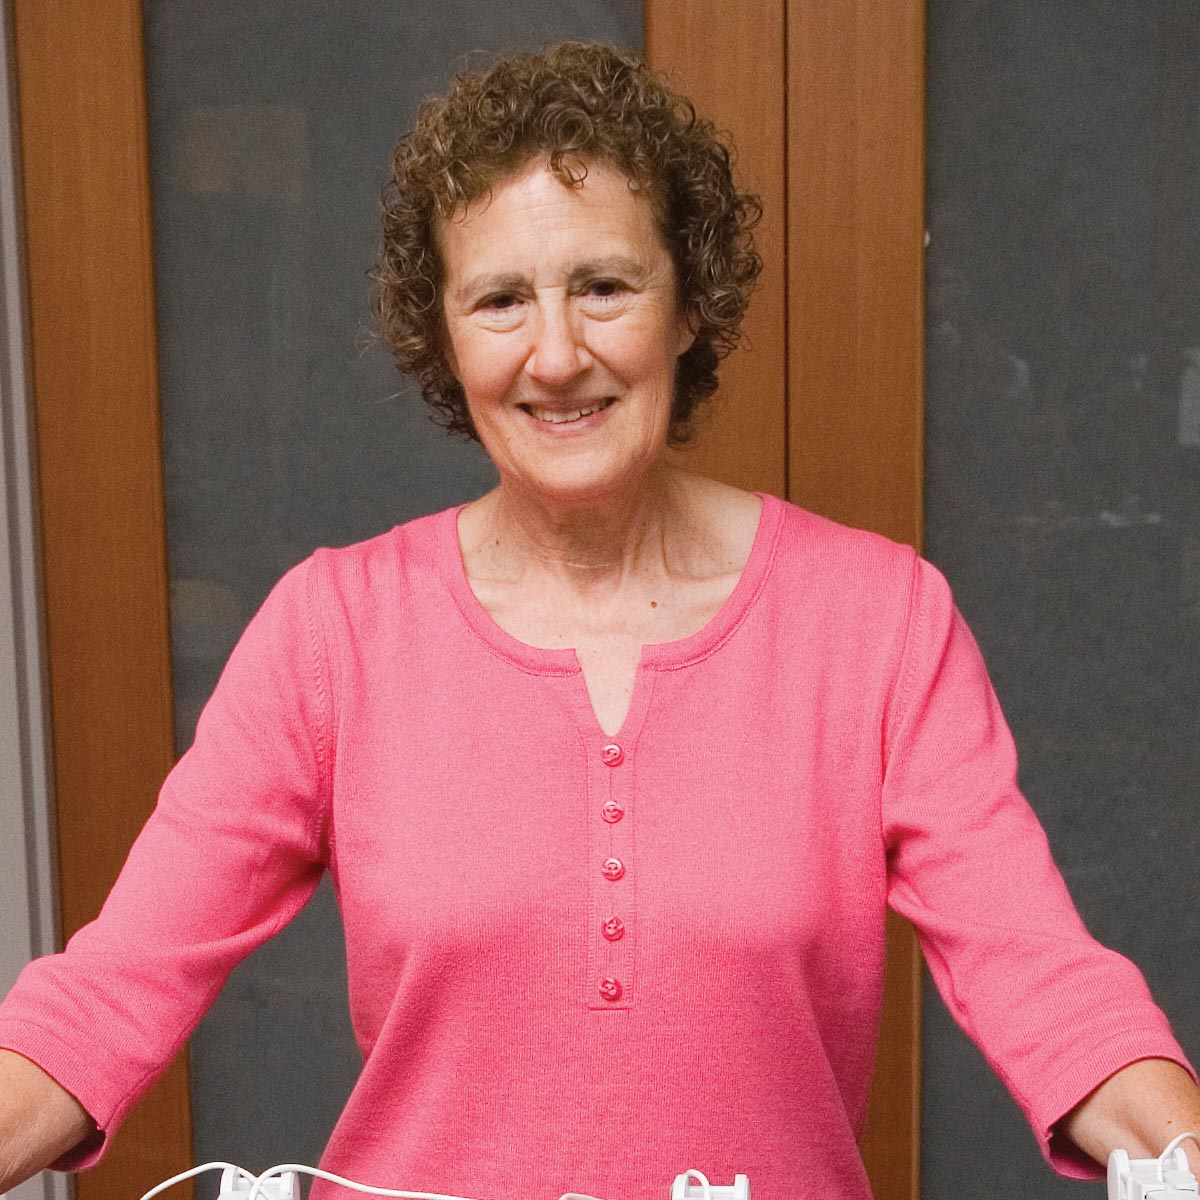
\includegraphics[scale=0.08]{fig/barbara-liskov}

\end{columns}
\begin{itemize}
	\item 2004 John von Neumann Medal winner for "fundamental contributions to programming languages, programming methodology, and distributed systems"
	\item 2008 Turing Award winner, for her work in the design of programming languages and software methodology that led to the development of object-oriented programming
\end{itemize}
\end{frame}

\begin{frame}[allowframebreaks]{Sub types and Liskov Substitution Rule}
The substitution rule is formally described as follows:
\begin{center}
 If $S$ is a subtype of $T$, then objects of type $T$ may be replaced with objects of type $S$ (i.e. an object of type $T$ may be substituted with any object of a subtype $S$) without altering any of the desirable properties of $T$ (correctness, task performed, etc.)
\end{center}
This is by all means very abstract. We provide a more "concrete" explanation.

\begin{center}
	\structure{Subtype relation is an ``IS-A" relationship.}
\end{center}

For examples, a \texttt{Swan} \alert{is a} \texttt{Bird}, thus a \texttt{class Swan} is a subtype of \texttt{class Bird}. A bird can fly, can quake and can lay eggs. A swan can also do these. It might do these better, but as far as we are concerned, we don't care. \texttt{Bird} is the super-type of the \texttt{Swan}.
\end{frame}

\begin{frame}{Pre-conditions \& Post-conditions}
The term ``sub-type" is misguiding because the prefix ``sub" suggests the sub-type is ``inferior" to the super-type in some sense. But this is actually other way around. 

\begin{itemize}
	\item The assertions in the \texttt{REQUIRES} clause and argument types in abstraction specs combined is called a ``Precondition".
	\item The assertions in the \texttt{EFFECTS} and \texttt{MODIFIES} clause specifies the post conditions. 
\end{itemize}

Sub-types typically perform a combination of belows:
\begin{itemize}
	\item Supports extra operation. Naturally preserves follows LSR.
	\item Weakens the pre-conditions. Expands range of input.
	\item Strengthens the post-condition. Enhances the effect.
\end{itemize}
In reality sub-types are beefed-up versions of the super-type. They perform more specific jobs or do the same job better.
\end{frame}

\begin{frame}[fragile]{Inheritance}
We now start to look at a specific language feature in C++, namely \textit{inheritance}. The syntax takes the form of the following:
\begin{minted}{c++}
class Derived : /* access */ Base1, ... {
    /* Contents of class Derived */
};
\end{minted}

When a class (usually called \textit{derived}, \textit{child} class or \textit{subclass}) inherits from another class (\textit{base}, \textit{parent} class, or \textit{superclass}), the derived class is automatically populated with \textit{everything} from the base class. \textit{Everything} includes member variables, functions, types, and even static members. The only thing that does not come along is \textit{friend}ship-ness, which is irony. 

Note that, it is one thing that the derived class ``has" everything from the base class, it is totally another thing whether the base class can access it. Whether the base class can access the member is dependent on the choice of \texttt{access}.
\end{frame}

\begin{frame}[fragile]{Inheritance access specifiers: \texttt{public}}
There are a three choices of \texttt{access}, namely \texttt{private}, \texttt{public} and \texttt{protected}. The most commonly used one is \texttt{public}. 

\begin{itemize}
	\item Private member of the base class stays private \textit{to the base class}. Even the derived class CANNOT touch them!
	\item Public member of the base class stays public. This means they are exposed as part of the interface of the derived class.
\end{itemize}

\inputminted[fontsize=\small]{c++}{code/rc10access/public.h}
\end{frame}

\begin{frame}[fragile]{Inheritance access specifiers: \texttt{private}}
When you omit the access specifier, the access specifier is assumed to be \texttt{private}. The \texttt{private} specifier follows the following rule. 

\begin{itemize}
	\item Private member of the base class stays private \textit{to the base class}. Same as before. 
	\item Public member of the base class are still accessible to the derived class. However they are no longer part of the interface of derived class. I.e. cannot be access from outside. 
\end{itemize}

\inputminted[fontsize=\small]{c++}{code/rc10access/private.h}
\end{frame}

\begin{frame}[fragile]{Member access specifiers: \texttt{protected}}
The first thing you need to hear about this keyword, is \textbf{DO NOT ABUSE IT}. Use it with extra care. The fact that base class private member is not accessible to derived class sometimes causes in convenience. We would like something that:

\begin{itemize}
	\item Not accessible by the outside world. 
	\item Accessible for derived class, if inherited as public. 
\end{itemize}

The key word that satisfies such need is \texttt{protected}.
\inputminted[fontsize=\small]{c++}{code/rc10access/protected.h}

We would really like to restrain ourself from using the keyword, since allowing other class to access a private comes with the possibility of the other class breaking invariants.
\end{frame}

\begin{frame}{Two aspects of inheritance}
There are two aspects of inheritance, namely:

\begin{block}{Inheritance of code: reusing code}
The derived class now comes with the same set of ``code", or contents of the base class. This essentially saves us time and effort of coding same thing again and again. 
\end{block}

\begin{block}{Inheritance of interface}
With public inheritance, the derived class will have the same interface (well, at least same method signatures...) as the base class. If used corrected, this creates a \textit{subtype}. 
\end{block}

Private inheritance is sometimes referred as \textit{implementation inheritance}, since it allows the derived class can reuse the code of the base class (as if the base class is a private member variable of derived class), without exposing the base class.

\textbf{We will assume public inheritance in the rest of this chapter. }
\end{frame}

\begin{frame}[fragile]{Remark: Inheritance \& subtyping}
There are two remarks that I would like to make. First of all, subtypes does not have to be created from inheritance. In the following code, class B is definitely a subtype of class A.

\begin{minted}{c++}
class A {public:void quak(){puts("Hello.");} };
class B {public:void quak(){puts("Hello.");} void nop();};
\end{minted}

On the other hand, having identical interface (or inheritance) does not guarantee subtyping relation. For example (why?):

\begin{minted}{c++}
class A { protected: int a = 0; 
          public:    int add(int i){ return i + a;} };
class B : public A { public:  B() : a(10) {} };
\end{minted}

Although inheritance is neither a sufficient nor a necessary condition of subtyping relation, it IS the only subtyping method supported by C++ (without a hack) in runtime. We will see this shortly after. 
\end{frame}

\begin{frame}[fragile]{Pointer, reference and sub classing}
From our previous discussion we see that there is no definite rule between a class being as subclass and a class being a subtype. However, from the language perspective, C++ simply \textbf{trusts} the programmer that every subclass is indeed a subtype. This is visible from the following rules:

Suppose we have \texttt{class Base} and \texttt{class Derived}, with \texttt{Derived} being a subclass of \texttt{Base}. We have the following rule.

\begin{itemize}
	\item Derived class pointer compatible to base class. 
	\item Derived class instance compatible to base class (possibly \texttt{const}) reference.
	\item *You can assign a derived class object to a base class object.
\end{itemize}

Two remarks. 1) The last rule needs further explanation. 2) Those rules are NOT true if reversed. For example, you cannot (normally) assign a base class object to derived class object. Assigning a base class pointer to derived class pointers needs special casting. 

\end{frame}

\begin{frame}[fragile]{Pointer, reference and sub classing: Example}
Code in \texttt{code/rc10compatible}
\twocolumncodenamed{code/rc10compatible/class.h}{code/rc10compatible/class.cpp}
\end{frame}

\begin{frame}{Pointer, reference and sub classing: The third rule}
Now the previous example demonstrates the first two roles. We know how things worked with reference and pointers. To explain the third rule, we need to understand first how synthesized methods worked with inheritance. Note that here we mainly focus on how copy constructors works. The case for the assignment operator overload is very similar.

Here we will use the following base class as an example:
\inputminted[fontsize=\small]{c++}{code/rc10synthesize/base.h}

Code in \texttt{code/rc10synthesize}
\end{frame}

\begin{frame}[fragile]{Pointer, reference and sub classing: Synthesized methods}
\vspace{-0.1in}
\inputminted[fontsize=\small]{c++}{code/rc10synthesize/ok.cpp}
A synthesized copy constructor will do things almost identical to synthesized default constructor. 
\begin{itemize}
	\item \textbf{Copy construct} the base class. See \texttt{Derived1}.
	\item \textbf{Copy construct} every member, if there is any. 
	\item Call the copy constructor of the class. 
\end{itemize}
The case of \texttt{Derived2} shows how we do this manually.
\end{frame}

\begin{frame}[fragile]{Pointer, reference and sub classing: Synthesized methods II}
\vspace{-0.1in}
\inputminted[fontsize=\small]{c++}{code/rc10synthesize/error.cpp}
Here are mistakes that people usually make. Without default constructor (\texttt{Derived3}), since you already provided a constructor, compiler won't synthesize default constructor for you! Without copy constructing the base (\texttt{Derived4}), the compiler will treat it as if the cpctor is a usual constructor, defaulting constructing the base and all members.
\begin{itemize}
	\item
\end{itemize}
\end{frame}

\begin{frame}[fragile]{Pointer, reference and sub classing: Copying}
Code in \texttt{code/rc10compatible}
\twocolumncodenamed{code/rc10compatible/class.h}{code/rc10compatible/copy.cpp}
\end{frame}

\begin{frame}[fragile]{Digression: Inheritance and memory map}
We now digression to the question of how does this work exactly. If we print the address of the objects in our previous example:
\begin{minted}{c++}
void addr1() {Derived d;  Base* b = &d; cout << b; }
void addr2() {Derived d;  Base& b = d; cout << &b; }
\end{minted}
You will see the same address being printed over and over again. Consider a function a function taking an base class pointer as argument. The function will have no idea the address passed to it, is indeed a base class object, or a derived class object ``disguised" as a base class object. 

The derived class object always ``embeds" a base class object at the begging of its corresponding memory region. Memory layout of Derived object looks like below.  
\begin{minted}{c++}
struct Derived { Base base; /* Derived members */ };
\end{minted}
This also explains why base class objects are initialized as if they are member variables, because to a degree they are!
\end{frame}

\begin{frame}{Introducing new methods to create subtypes}
Now we go back to the question of subtypes. Recall the 3 three ways of creating subtypes. Two  involves modifying existing methods. The last one involves adding extra operations. Adding extra operations is simply adding methods to the derived class.  

\begin{block}{The term ``sub-type" is misleading?}
Adding new methods usually enhances the class, yet the enhanced version is called a ``sub-type", as if it is inferior in functionality. However, the derived class is not only \textit{enhanced}, but also \textit{specialized}. It is less general than its superclass, which is ``sub-".
\end{block}

\begin{block}{Should I use ``protected"?}
If there is no shared data between derived class and base class, e.g. global variables, protected member, static members etc, adding a new method always results in a sub type. Though sometimes you want share some data structure.... Be careful!
\end{block}
\end{frame}

\begin{frame}[fragile]{First (failed) attempt towards new sub-typing}
We now make an attempt of the the other two ways of subtyping. Both relaxing preconditions or tightening postconditions requires modifying existing methods. Since we cannot modify existing functions, our naive attempt is to define a function with the same name as the function being modified, hoping that this function would somehow ``replace" the original function. 

Consider the following example from your lecture slides. Suppose we have an \texttt{IntSet} and \texttt{SortedIntSet}.

\begin{minted}{C++}
class IntSet { 
protected: int count, *data; 
public: /* Other methods ommited */
  void insert(int i) {cout << "IntSet\n"; ... } };
class SortedIntSet : public IntSet { public: 
  int  max() { /* Get maximum (last) element */ }
  void insert(int i) {cout << "SortedIntSet\n"; ...} };
\end{minted}
\end{frame}

\begin{frame}[fragile]{First (failed) attempt of sub-typing, Con't}
\begin{minted}{C++}
void test1() { 
    SortedIntSet set; 
    /* A number of insert / del / max */ }
void insert100(IntSet& set) { set.Insert(100); }
void test2() { 
    SortedIntSet set; set.insert(10); 
    insert100(set);  /* Will print IntSet */
    cout << set.max() << endl; /* very likely be 10 */ }
\end{minted}

When you run functions like \texttt{test1()}, everything will be fine. You cannot break things if you just stick with functions like \texttt{test1()}. However, when you do function \texttt{insert100()}, a function that assumes sub-typing, you might break your instance's invariance!

Breaking the invariance is bad. We know that very well. But we need to look closer. We must ask, how did we fail? And what exactly are the damage?
\end{frame}

\begin{frame}[fragile]{Static binding causes the problem}
Recall how C++ links member function calls?
\begin{itemize}
	\item All member functions are just usual functions.
	\item When a member function call happens, the compiler links the function according to the type of the class instance, passing the object as the first argument. 
\end{itemize}

Now in \texttt{insert100()}, the method  \texttt{insert()} is called on object \texttt{set}. \texttt{set} is an instance of \texttt{IntSet}. In this case, the compiler will choose the function \texttt{IntSet::Insert()}. 
Remember that the compiler have no idea what is actually referenced by \texttt{set}. When it compiles \texttt{insert100}, all it knows is that \texttt{set} refer to an object of \texttt{IntSet}. It doesn't care if this object is part of a larger object. 

In fact, up till this point, when you make a function call in the code, the actual function being called is always know at compile time. \textbf{The process of binding a function call to the actual definition is \textit{static}. }
\end{frame}

\begin{frame}[fragile]{Name hiding}
On the other hand, you could always:
\begin{minted}{c++}
void test3() {
  SortedIntSet set; set.insert(10; /* SortedIntSet */
  IntSet& is = set; set.insert(10); /* IntSet */)}
\end{minted}

Using a simple reference, you can always access the function you should have replaced. In fact, the \texttt{SortedIntSet} actually exposed 2 sets of interfaces:
\begin{itemize}
	\item \texttt{IntSet::insert(int)}, inherited from \texttt{IntSet}.
	\item \texttt{SortedIntSet::insert(int)}, which is defines.
\end{itemize}

Defining a method with same DOES NOT replace the original function. Instead, it only adds a new function! It's just when you say \texttt{insert()}, the compiler has two choices. Instead of complaining,   it chooses the ``closest" match. The second function ``hides" the name of the first one. This is called \textit{name hiding}. You can expose the first one with a \texttt{using} statement.
\end{frame}

\begin{frame}[fragile]{Name hiding is not sub-typing (in general)}
\begin{itemize}
	\item \texttt{IntSet::insert(int)}, inherited from \texttt{IntSet}.
	\item \texttt{SortedIntSet::insert(int)}, which is defines.
\end{itemize}
We finally examine the damage. How bad is the name hiding? 
\begin{itemize}
	\item First of all, substitution rule still works here. Replacing \texttt{IntSet} with \texttt{SortedIntSet} will not break any existing code. So \texttt{SortedIntSet} is (arguably!) a subtype of \texttt{IntSet}.
	\item We can also think in terms of invariants. All methods exposed by a class must always maintain invariance. In our case \texttt{SortedIntSet} assumes a different set of invariance (the ordering),  \texttt{IntSet::insert} will break the invariance. That's what actually goes wrong. 
	\item On the other hand, in this case \texttt{SortedIntSet::insert} will not break the invariance of \texttt{IntSet}. However, since two classes are sharing data, this will NOT be the case in general. If the \texttt{SortedIntSet::insert} breaks the invariance of \texttt{IntSet}, they will be no subtyping. 
\end{itemize}
\end{frame}

\subsection{Virtual-ness and runtime polymorphism}
\begin{frame}{The need for polymorphism}
Why are we spending so many time on the name hiding things. Well, the example motivates the following discussions. 
\begin{itemize}
	\item From the subtyping perspective, we want something that allows us to implement other two ways of subtyping. 
	\item As we have shown, doing this often requires actually ``replacing" the method call, not just hiding it. 
	\item For functions using that call, let's say \texttt{insert100}, the actual function being called would be dependent on what the reference actually is. The fact that identical code behaves differently for different object is called \textit{polymorphism}.
	\item We will only know that the actual object being referenced at runtime, which means the binding process must be dynamic, i.e. happens also in the runtime. What we want is a form of \textit{dynamic polymorphism}.
\end{itemize}
All that boils down to the what is known as \textit{virtual} functions.
\end{frame}

\begin{frame}{\textit{Apparent type} and \textit{actual type}}
Before we head out to define what virtual functions are we first start out to make two definitions:

\begin{description}[Apparent Type]
	\item[Apparent Type] Apparent type is the type annotated by the type system. It is the static type information. It is the you remarked to the compiler.
	\item[Actual Type] It is the data type of the actual instance. It is the data type that describes what exactly is in the memory.
\end{description}

In our previous example, in function \texttt{insert100()}, the apparent type of the variable \texttt{set} is \texttt{IntSet}, while what's in the memory is actually a \texttt{SortedIntSet} (The actual type).

If we note again we have discussed using these new term, normally C++ resolves function bindings based on apparent type. Since apparent types are always known at compile time, function binding will be able to be resolved at compile time. 
\end{frame}

\begin{frame}[fragile]{Dynamic \textit{polymorphism} through \textit{virtual}-ness}
What we want is dynamic function binding, the ability to bind a function call based on an object's actual type, instead of the apparent type. This is done through the \texttt{virtual} keyword. Using previous example:

\begin{minted}{c++}
class IntSet { /* ... */
public:  
    virtual void insert(int i) { /* Impl ommited */ }
};
\end{minted}

The above syntax marks \texttt{insert} as a \texttt{virtual function (method)}. Virtual methods are methods replaceable by subclasses. When a method call is made, if the method you are calling is a virtual function (based on the apparent type), the language bind the call according to the actual type. In this way, the function \texttt{insert100} achieves dynamic polymorphism, the ability to change its behavior based on the actual type of the argument.
\end{frame}

\begin{frame}[fragile]{Inheritance and keyword \texttt{override}}
\vspace{-0.1in}
Virtual functions are functions that allows being replaced by subclasses. This is done by the subclass defining a function with identical name as the base class. 
\begin{minted}{c++}
class SortedIntSet : public IntSet {
public: void insert(int i) { ... } ...  };
\end{minted}
The act of replacing a function is called \textit{overriding} a base class method. As you can imagine, if you somehow forgot the \texttt{virtual} keyword in the base class, overriding would become name hiding, which is subtle but dangerous. C++ provides a keyword to allows make clear your intent:
\begin{minted}{c++}
void insert(int i) override { ... }
\end{minted}
Would cause the compiler to verify if a function is indeed overriding a base class method. If the base class method is not a virtual function, compiler will complain. The keyword is introduced in C++11. \textbf{It is considered a best practice always mark override whenever possible}.
\end{frame}

\begin{frame}[fragile]{Fix our example with \texttt{virtual}}
With the changes we have noted, now this is fine
\begin{minted}{c++}
void insert100(IntSet& set) { set.Insert(100); } /*same*/
IntSet is; insert100(is);          /* print 'IntSet' */
SortedIntSet sis; sis.insert(10);
insert100(sis); cout << sis.max(); /* SortedIntSet; 100 */
\end{minted}

Now when \texttt{set.Insert()} is called inside \texttt{insert100}, the apparent type is still \texttt{IntSet}. however, the compiler finds out that \texttt{insert} is a virtual method. Thus it generates code that makes the call based on the actual time at runtime.

At runtime, when \texttt{IntSet} instance is passed, the actual type is just \texttt{IntSet}, so it binds it \texttt{IntSet::insert()}. The other situation, the actual type is  \texttt{SortedIntSet}, so it binds it to \texttt{SortedIntSet::insert()}. Now what if modify \texttt{insert100} to?
\begin{minted}{c++}
void insert100(IntSet /*byVal*/ set) {set.Insert(100);}
\end{minted}
\end{frame}

\begin{frame}[fragile]{Inheritance and keyword \texttt{final}}
On the other hand, \textit{virtualness is automatically inherited}. For instance, if have class and another function:

\begin{minted}{c++}
class QuickSortedIntSet : public SortedIntSet { ...
public: void insert(int i) { ... } };
void insert200(SortedIntSet& set) {set.Insert(200);}
\end{minted}

You DO NOT need to change \texttt{SortIntSet} to achieve below:

\begin{minted}{c++}
QuickSortedIntSet qsis; 
insert100(qss); insert200(qss); /* QuickISIS*/
\end{minted}

Sometimes, for instance, \texttt{SortedIntSet} would like to stop its methods being override by further subclass (Why?). In this case, you can mark its method using the keyword \texttt{final}. 

\begin{minted}{c++}
/* SortedIntSet */ void insert(int) override final {...}
\end{minted}
The order of two keyword does not matter. Trying to override a method with \texttt{final} causes compilation error. 
\end{frame}

\begin{frame}[fragile]{Remark: Use overriding with extra care}
The overriding mechanism provides the programmer with a mechanism to change the \textbf{base} class behavior. The emphasis is that you not only able to modify your own class, \textit{you would also be able to modify the behavior of another class, with it knowing it!} It sounds dangerous, and you make make careful use of it. 

First of all, overriding not always creates subtypes. For instance if we override \texttt{IntSet::insert()} with an the following:

\begin{minted}{c++}
/* SortedIntSet */ void insert(int) override {numElts--; }
\end{minted}

This function will very likely break the invariant of \texttt{IntSet}. The substitution would fail, and there goes the sub typing relations.
\end{frame}

\begin{frame}{Reuse of implementation and object composition}
Secondly, virtual methods are almost the most misused feature of C++! We have noted inheritance has two affects: reuse of implementation and interface. Many would ``accidentally" involve the latter, while what they actually want the first! 

If you just want the implementation, there are two ways to go:
\begin{itemize}
	\item Private inheritance, as we have discussed before,
	\item Or even better, declare the base class object as a member instead of deriving from it. This is called \textit{composition}.
\end{itemize}

Let's take a look at an example:

Suppose we have a \texttt{class Graph} that abstracts the concept of a graph. It supports \texttt{Graph::InsertNode(string name)} and \texttt{Graph::addEdge(string node1, string node2)}. Suppose we have a class \texttt{Binary} tree that inherits \texttt{Graph}. It supports one more operation \texttt{Tree::GetRoot()}. The question is whether \texttt{Tree} is a sub-type of \texttt{Graph}?
\end{frame}


\begin{frame}{Remark: Differentiating \texttt{IS-A} and \texttt{HAS-A}}
Unfortunately the answer is negative. The reason should be obvious. There is essentially no requirement on where the edges and nodes are (precondition is weak). But you can't add arbitrary edges and nodes must connect to at most 2 other nodes (stronger precondition). \alert{So a \texttt{Tree} is not a  \texttt{Graph} in the subtype sense}.

\vspace{0.1in}
However we would naturally see that a \texttt{Tree} type must have a lot common code as the \texttt{Graph}. We would like to avoid rewriting them. There are two ways to do this:
\begin{itemize}
	\item Through \texttt{private} inheritance (implementation inheritance). We would not discuss this.
	\item By setting \texttt{Graph} as a member of a \texttt{Tree} type. We forward calls to \texttt{Graph}. This is a typical case of a \texttt{Has-A} implementation.
\end{itemize} 
\end{frame}

\begin{frame}{Compiling technology supporting virtualness}
\textit{Note we are now in the field of undefined behavior.} We are now going to discuss how virtual functions are implemented internally. Knowing this will help you solve exam questions. However, what we are going to discuss here are not ground truth. I.e. things could change from platform to platform. 

Internally, virtual functions are implemented using VTables:

\begin{itemize}
	\item Virtual methods are grouped together in an array of function pointers, as if they are member variables. This array is called \textit{Virtual Table}, or \textit{vtable} 
	\item When the compiler makes a virtual method call, it calls the function pointer in the corresponding entry of the vtable. 
	\item When derived objects instantiates itself, it replaces entries of function it need to override in the vtable, with its own implementation.
\end{itemize}
\end{frame}

\begin{frame}{Virtual Tables and performance: No free lunch}
\vspace{-0.1in}
Virtual function comes with preformance hit
\begin{itemize}
	\item The cost of one extra layer of indirectness. There exists one more pointer dereference to find the target function. That's one more memory access. 
	\item Cost of unknown call target. Modern processors will ``prefetch", or guess the future instructions and execute them in advance. Since the function call target is unknown, this will not be possible for virtual functions
	\item Cost of unable to inline methods. For simple methods, compiler will try to inline them. Since the binding happens at runtime for virtual methods, this is no longer possible.
\end{itemize}
Using the \texttt{final} keyword will help. If the compiler is able to determine the actual type, it may choose to preform \textit{de-virtualization}. Those costs could be quite huge if the method is used frequently. In old time the cost is often indurable. Modern computers are more powerful, things get better.
\end{frame}

\begin{frame}[fragile]{Using VTable to solve problem}
\twocolumncodenamed{code/rc10virtual/class.h}{code/rc10virtual/call.cpp}
\end{frame}

\begin{frame}[fragile]{Using VTable to solve problem}
\begin{columns}
	\column[]{.5\textwidth}
	
	The idea will be to draw out the VTable for each object. E.g. When you run \texttt{b1.h()}, you would find that the apparent type of \texttt{b1} is \texttt{Bar}. And \texttt{Bar} does not have an entry for \texttt{h()}. So this is static linkage. On the other hand, if you run \texttt{b2.h()}, \texttt{b2} is \texttt{Baz}. We thus follow the vtable to find the function call.

	
	\column[]{.5\textwidth}
	
	Vtable for \texttt{Qux} instance:
	\inputminted[fontsize=\small]{c++}{code/rc10virtual/vtable_qux.cpp}
\end{columns}
\end{frame}

\begin{frame}[fragile]{Pure virtual functions and classes}
It is possible that we do not supply a implementation when defining a base class. In this case, the corresponding entry in the vtable would simply be left unfilled:

\begin{minted}{c++}
/* IntSet */ virtual void insert(int i) = 0;
\end{minted}

In this case we say the method is \textit{pure virtual}. If a class contains \textbf{one or more} pure virtual methods, we say the class is a \textit{pure virtual class}. You only need to have one pure virtual function for a class to be ``purely virtual".

You \textbf{CANNOT} instantiate a \textit{pure virtual class}. This is somewhat obvious. If you ever have an instance of \texttt{IntSet}, what should happen when you call \texttt{IntSet::insert()}?

Pure virtual class are also called \textit{abstract base classes}, or \textit{interfaces}. We will explain this terminology shortly after. It is often that the name abstract base classes starts with a case letter \texttt{I} (/ai/) for \textit{interface}.
\end{frame}

\begin{frame}[fragile]{Abstract base classes}
Why would we ever wanted a pure virtual classes since we cannot instantiate it? Because we would want to model abstract \textit{concepts}. We would like to say things like \textit{Matricies are subclass of summable object}. We would like to increase code reuse. Consider the following class:

\begin{minted}{c++}
class ISummable { public: 
    /* Add item x to itself */
    virtual void add(ISummable& x) = 0; };
\end{minted}

This class models the objects that are summable. Based on this modeling, we could write the following very general function:

\begin{minted}{c++}
void sum(ISummable elem[],size_t size, ISummable& rst) {
    for (int i = 0; i < size; ++i) rst.add(elem[i]); }
\end{minted}

This will work for anything that is \texttt{Summable} object. When a class derives from an interface and provides an implementation, we say it \texttt{implements} the interface. 
\end{frame}

\begin{frame}[fragile]{Programming with interfaces}
Abstract base classes provides very strong decoupling technique, in a large project:
\begin{itemize}
	\item One team of engineers write algorithms using the interface.
	\item Another, independent team of engineer write classes that implements the interface.
	\item The only coupling point is the interface itself. Once the interface is agreed upon, two teams can work independently.
\end{itemize}
This is even better if you ever would like to update your code:
\begin{itemize}
	\item To support new features, simply write \textbf{more} classes. There is no need change any existing code. 
	\item To update existing feature, only rewrite and recompile the part related. I.e. you only recompile the algorithm, or the classes implementing the interface. 
	\item Dynamic linking technology, you could update your software by shipping the end user only \textbf{part} of the entire binary.
\end{itemize}
\end{frame}

\begin{frame}[fragile]{Programming with interfaces}
Modern software engineering technologies usually ``abuses" the Liskov Substitution rules by write software that depends only on interfaces. In this way maximum utilization is achieve. For instance, we now provide an example of what is known as \textit{``Factory" design pattern}. Let's say you are asked to write a encryption program that intends to support a number of ciphers. You first abstract out what a cipher is:

\begin{minted}{c++}
class EncryptionEngine {
public:
  virtual string name() = 0;
  virtual string generateKey() = 0;
  virtual string encrypt(...) = 0;
  virtual string decrypt(...) = 0;
  virtual ~EncryptionEngine() = default;
};
\end{minted}
\end{frame}

\begin{frame}[fragile]{Programming with interfaces, II}
Then you write a few engines, and write a \textit{factory method}:
\begin{minted}{c++}
EncryptionEngine *
encryptionEngineFactory(std::string engine) {
  engine =string_tolower(engine);
  if (engine == "aes") return new AesEngine;
  if (engine == "rc6") return new Rc6Engine;
  if (engine == "dummy") return new DummyEngine;
  throw UnknownEngine(engine);
}
\end{minted}

In the main,  use a \texttt{unique\_ptr} to preform memory management.

\begin{minted}{c++}
string algorithm = getEngineName();
unique_ptr<EncryptionEngine> engine(
  encryptionEngineFactory(algorithm)
); cout << engine->enrypt("abc", "DEADBEEF");
\end{minted}
\end{frame}

\begin{frame}[fragile]{Programming with interfaces, III}
\vspace{-0.1in}
This method gives you a number of advantages:
\begin{itemize}
	\item First of all, it allows you to decouple the encryption algorithm from the code that handles you user input. The user input may come from GUI, input or a file. We simply don't care. The main routine would be exactly the same
	\item Then, you no longer need to duplicate any code to support more algorithms. This prevents possible mistakes.
	\item Finally, this gives you the flexibility of dynamically add, remove, disable, enable some algorithms. You could complicate your factory methods, for instance, check if your user have paid for your program. The list of available engines could come from Internet, or from a configuration file. 
\end{itemize}
\end{frame}

\begin{frame}{Remark on \textit{design patterns}}
\begin{columns}
	\column[]{.5\textwidth}
	
There exists a number (over 20) of different (object oriented) design patterns. The urge for design pattern rise with the popularizing of JAVA. Almost all of them relies on interfaces. There exists a book written by GOF called \textit{Design Patterns} listing all of them. The book is considered one of the most classical text book for software engineering. 
	
	\column[]{.5\textwidth}
	\vspace{-0.2in}
	\begin{center}
		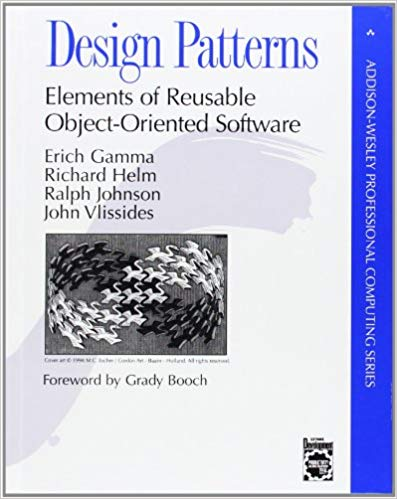
\includegraphics[scale=0.37]{fig/design_patterns.jpg}
	\end{center}
\end{columns}
\end{frame}

\begin{frame}{Is it a subtype?}
Designing whether something is or is not a subtype of a particular super type is probably in the heart of program structure design.

\structure{A Remark}

The problem of whether two objects form a ``IS-A" relation must be understood in a realistic context. Consider two classes \texttt{RegularIntSet} and \texttt{SortedIntSet}. Suppose both of them supports a \texttt{max()} function.
\begin{itemize}
	\item You can argue that \texttt{RegularIntSet} is a sub-type of \texttt{SortedIntSet} because they support the same set of operations.
	\item You can also claim that \texttt{RegularIntSet} is NOT a sub-type since the \texttt{max()} of \texttt{RegularIntSet} is significantly slower than it's counterpart. One could argue the performance is part of the abstraction.
\end{itemize}
\end{frame}


